\section{Vulnerable Reconstruction and Controlled Reproduction}
\label{sec:controlled-reproduction}

\graphicspath{{../evidence/}{evidence/}}

Chapter~4 established that VM~270 was already protected and could not serve as
the direct reproduction target. The active kernel was beyond Canonical's fixed
package boundary, and the ordinary \code{modprobe} path for
\code{algif\_aead} was blocked. VM~270 therefore remained the reference
system. The vulnerable state was reconstructed on VM~271
\code{copyfail-vuln}, the separate experimental clone created for this phase.

The reconstruction used Ubuntu kernel \code{6.8.0-116-generic}, supplied by
package version \code{6.8.0-116.116}. Before the preserved execution, the
running kernel, package state, module-loading path, test identity, and selected
SUID target were recorded. The proof of concept was then launched from
\code{labuser}, UID~1001. Success was defined by the resulting process
reporting UID~0, not by a changed prompt or file digest alone.

A preliminary run had already been used to explore the behaviour of the target
file. Because that run changed the byte stream returned through the mounted
path, VM~271 was rebooted into the same vulnerable kernel before the preserved
sequence began. The final run therefore starts from a restored observable
target state instead of presenting an already modified system as clean.

No persistence, credential collection, lateral movement, reverse shell, or
unrelated post-exploitation activity was performed. The chapter follows the
experiment only as far as necessary to establish the UID transition, compare
the two observed file-access paths, and record recovery after reboot.

\begin{evidencebox}
Phase~02 is stored under \path{evidence/02-reproduction/}. Its manifest lists
12 objects: five text artifacts, six screenshots, and the phase README. All 11
experimental captures verify against \path{PUBLIC-SHA256SUMS}; only the listed
\path{README.md} digest is stale. The README is therefore used as supporting
documentation, not as an integrity-verified experimental object. Screenshot
ID~04 remains intentionally absent because it exposed the complete
proof-of-concept source.
\end{evidencebox}

\subsection{Experimental Boundary and Evidence Sequence}

The evidence set contains two related but distinct sequences. The preliminary
investigation is represented by
\path{artifacts/copyfail-confirmed-vulnerable-state.txt}. It records the
intended historical kernel and package versions, the required modules in the
loaded state, and a mounted-view target digest that had already changed. That
artifact is useful for confirming the reconstructed runtime, but it cannot be
used as the clean before-state for the final execution.

VM~271 was therefore rebooted before the preserved run. It returned to
\code{6.8.0-116-generic}, and the normal mounted path for
\code{/usr/bin/su} again produced the original comparison digest:

\begin{lstlisting}
c74311fe5636b7d7f9a56239fa8adeeab12ba86fe7d41b91afa85bf9bbdae78b  /usr/bin/su
\end{lstlisting}

Here, \emph{restored observable state} means that the same vulnerable kernel
was active and the selected target again matched its recorded metadata and
mounted-view digest. It does not claim that every byte or item of volatile VM
state was compared with the original clone.

The retained evidence then follows the order shown in
\cref{tab:phase02-sequence}.

\begin{table}[H]
    \centering
    \caption{Preserved Phase~02 evidence sequence.}
    \label{tab:phase02-sequence}
    \small
    \begin{tabularx}{\textwidth}{@{}>{\bfseries}p{0.07\textwidth}>{\raggedright\arraybackslash}p{0.25\textwidth}Y@{}}
        \toprule
        ID & Preserved form & Role in the experiment \\
        \midrule
        01 & Text and screenshot &
        Records the vulnerable kernel, UID~1001 test account, SUID target, and
        original target digest before execution. \\

        02 & Screenshot &
        Records \code{algif\_aead} and \code{af\_alg} in the loaded state
        used for the reproduction. \\

        03 & Screenshot &
        Records proof-of-concept execution, the UID~0 shell, and the changed
        digest returned through the mounted target path. \\

        04 & Intentionally omitted &
        The original screenshot exposed the complete proof-of-concept source
        and is not part of the public package. \\

        05 & Text and screenshot &
        Records the return to UID~1001 while the changed mounted-view digest
        remained observable. \\

        06 & Text and screenshot &
        Compares the mounted/VFS digest with a direct read from the backing
        ext4 filesystem. \\

        07 & Text and screenshot &
        Records the original mounted-view digest after rebooting into the same
        vulnerable kernel. \\
        \bottomrule
    \end{tabularx}
\end{table}

The absent ID~04 remains in the numbering so the public files still match the
original collection order. IDs~02 and~03 are screenshot-only records; the other
retained steps also have machine-readable text. That difference matters. The
manifest verifies the published screenshot bytes, but it cannot turn a terminal
image into independently executable output or recreate the omitted source.

\subsection{Reconstructed Runtime and Clean Starting State}

The preliminary runtime capture reports the following active release and
matching package versions:

\begin{lstlisting}
6.8.0-116-generic
linux-image-6.8.0-116-generic          6.8.0-116.116
linux-modules-6.8.0-116-generic        6.8.0-116.116
linux-modules-extra-6.8.0-116-generic  6.8.0-116.116
\end{lstlisting}

The agreement between the booted release and the installed image and module
packages shows that the historical kernel was not merely present beside a newer
runtime. It was the kernel active during the experiment. Version
\code{6.8.0-116.116} is immediately before Canonical's first corrected Noble
generic package, \code{6.8.0-117.117} \cite{ubuntu-copyfail-cve}. The later
execution provides the behavioural confirmation that this reconstructed state
remained exploitable under the laboratory conditions.

Evidence item~01 was captured at \code{2026-08-08 23:02:32 UTC}, after the
reboot and before the final proof-of-concept execution. It records:

\begin{table}[H]
    \centering
    \caption{Observable starting state of the preserved run.}
    \label{tab:phase02-pre-exploit-state}
    \small
    \begin{tabularx}{\textwidth}{@{}>{\bfseries\raggedright\arraybackslash}p{0.30\textwidth}Y@{}}
        \toprule
        Observation & Recorded value \\
        \midrule
        Running kernel & \code{6.8.0-116-generic} \\
        Test identity & \code{uid=1001(labuser)}, \code{gid=1001(labuser)} \\
        Supplementary group & \code{100(users)} \\
        Selected target & \code{/usr/bin/su} \\
        Target metadata & \code{-rwsr-xr-x root root 55680} \\
        Mounted-view digest &
        \texttt{c74311fe...bbdae78b} \\
        Loaded AF\_ALG modules & No matching rows returned \\
        \bottomrule
    \end{tabularx}
\end{table}

\begin{figure}[H]
    \centering
    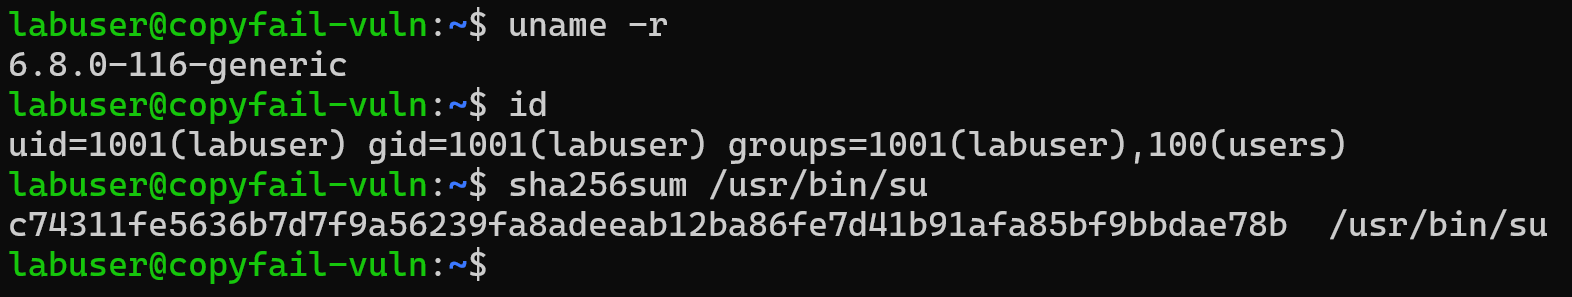
\includegraphics[
        width=\textwidth,
        height=0.25\textheight,
        keepaspectratio
    ]{02-reproduction/screenshots/01-pre-exploit-state.png}
    \caption{Interactive pre-exploitation capture showing the vulnerable
    kernel, UID~1001 test identity, and original mounted-view digest.}
    \label{fig:phase02-pre-exploit}
\end{figure}

The associated text artifact supplies the target metadata and collection time
that are not visible in the screenshot. It also records an empty exact-name
module query followed by the ordinary dry-run resolution:

\begin{lstlisting}
insmod /lib/modules/6.8.0-116-generic/kernel/crypto/af_alg.ko.zst
insmod /lib/modules/6.8.0-116-generic/kernel/crypto/algif_aead.ko.zst
\end{lstlisting}

Unlike VM~270, this path contains no \code{install /bin/false} replacement.
The empty runtime result therefore meant \emph{unloaded but normally loadable},
not absent or blocked through the tested \code{modprobe} path. The dry run did
not load either module. Evidence item~02 records the subsequent preparation
step performed by the administrative \code{researcher} account:

\begin{figure}[H]
    \centering
    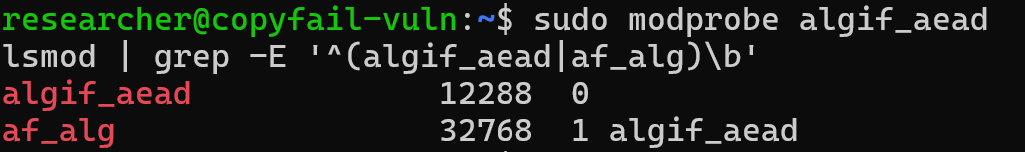
\includegraphics[
        width=\textwidth,
        height=0.20\textheight,
        keepaspectratio
    ]{02-reproduction/screenshots/02-algif-aead-loaded.png}
    \caption{Laboratory preparation step loading \code{algif\_aead} and
    recording its \code{af\_alg} dependency before exploitation.}
    \label{fig:phase02-modules-loaded}
\end{figure}

This administrative module load is not the privilege escalation. It establishes
the interface state required by the experiment, while the proof of concept was
launched separately from the \code{labuser} session. The screenshot proves the
loaded module state, not a complete AEAD encrypt/decrypt round trip.

\subsection{Proof-of-Concept Execution and UID~0 Transition}

Evidence item~03 begins at the ordinary-user prompt and records the decisive
execution sequence:

\begin{lstlisting}
labuser@copyfail-vuln:~$ python3 ~/copy_fail_exp.py
# id
uid=0(root) gid=1001(labuser) groups=1001(labuser),100(users)
# whoami
root
\end{lstlisting}

\begin{figure}[H]
    \centering
    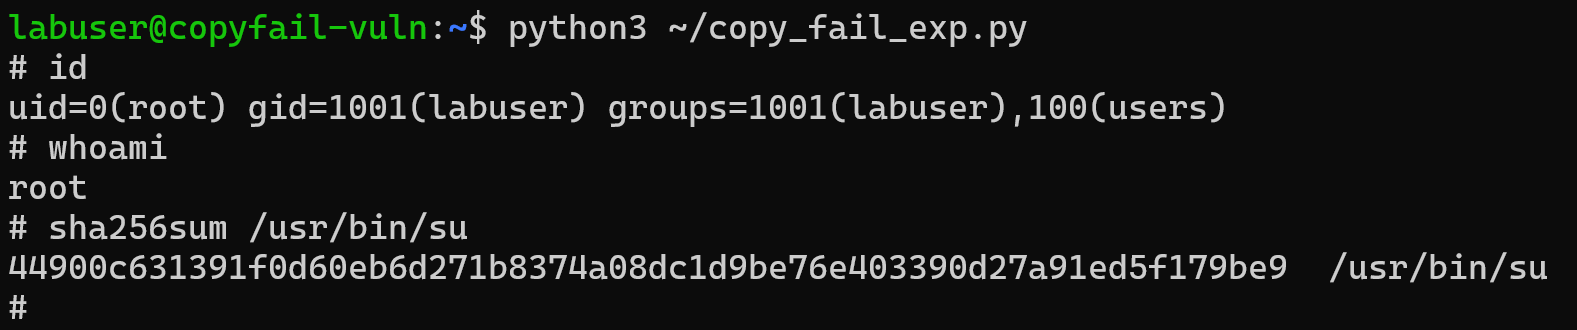
\includegraphics[
        width=\textwidth,
        height=0.28\textheight,
        keepaspectratio
    ]{02-reproduction/screenshots/03-privilege-escalation-success.png}
    \caption{Preserved execution showing the transition from the
    \code{labuser} prompt to a shell whose identity checks return UID~0 and
    \code{root}.}
    \label{fig:phase02-uid0-transition}
\end{figure}

The execution command is shown without \code{sudo}, \code{su}, or another
explicit privilege-granting wrapper. The change from a \code{\$} prompt to a
\code{\#} prompt is visually consistent with privilege, but it is not the
success criterion. The direct \code{id} and \code{whoami} results establish
the UID~0 process identity.

The process retained GID~1001 and the displayed group memberships of
\code{labuser}. The result is therefore described precisely as a transition to
UID~0, not as replacement of every credential field with the conventional root
account state. UID~0 is the trust-boundary crossing defined in Chapter~1 and is
sufficient to demonstrate local privilege escalation in this experiment.

The same screenshot records a changed SHA-256 digest for the mounted path:

\begin{lstlisting}
44900c631391f0d60eb6d271b8374a08dc1d9be76e403390d27a91ed5f179be9  /usr/bin/su
\end{lstlisting}

That changed digest is supporting behavioural evidence, not the proof of
privilege escalation. It shows that the bytes returned through the mounted path
differed from the before-state, but it does not identify the changed bytes or
prove a persistent replacement on disk.

The complete proof-of-concept source is not redistributed. Public evidence ID~04
was removed because it displayed the full source, while the numbering and
documentation retain the fact that the item existed. The Phase~02 documentation
records a 731-byte local representation and its SHA-256 digest, plus a
non-executed 732-byte trailing-newline variant. Because the README's manifest
entry is stale and item~03 does not hash the file immediately before launch,
those values are treated as documentation-level provenance rather than a
cryptographic binding between the screenshot and the exact executed bytes.

\subsection{State After Leaving the Root Shell}

Evidence item~05 was captured at \code{2026-08-08 23:24:57 UTC}, after the
UID~0 shell had been exited. The active session again reported
\code{uid=1001(labuser)} and \code{whoami} returned \code{labuser}. The target
still had the same size, owner, group, and SUID mode recorded before execution,
but its mounted-view digest remained changed.

\begin{figure}[H]
    \centering
    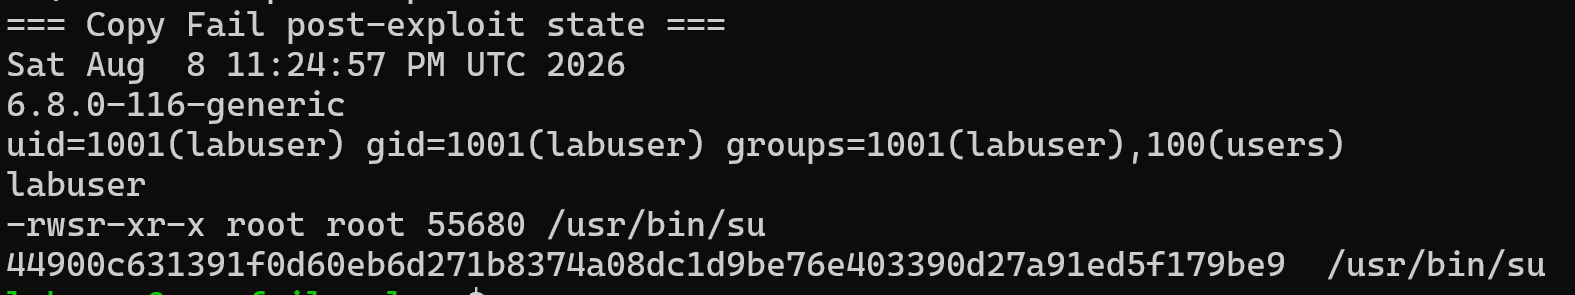
\includegraphics[
        width=\textwidth,
        height=0.26\textheight,
        keepaspectratio
    ]{02-reproduction/screenshots/05-post-exploit-state.png}
    \caption{Post-shell capture showing UID~1001 restored while the changed
    mounted-view digest remained observable.}
    \label{fig:phase02-post-exploit}
\end{figure}

Leaving the privileged shell therefore did not immediately restore the original
byte stream returned for \code{/usr/bin/su}. This does not establish persistence
in the usual security sense. No mechanism was installed to survive reboot,
retain privileged access, or automatically recreate the altered state. The
capture establishes only that the changed mounted view remained visible while
the system continued running.

The unchanged metadata also shows why a check limited to ownership, mode, and
size would not have detected the observed content difference. Conversely, a
changed digest cannot explain where the differing data resided or whether it
was ever written to persistent storage. The separate read-path comparison was
performed to answer that narrower question.

\subsection{Mounted View and Backing ext4 Read}

Evidence item~06 was captured at \code{2026-08-08 23:28:41 UTC}. The mounted
path was hashed again and compared with a direct read through \code{debugfs}
from the ext4 filesystem on the underlying logical volume:

\begin{lstlisting}
sudo debugfs -R 'cat /usr/bin/su' \
  /dev/mapper/ubuntu--vg-ubuntu--lv 2>/dev/null \
  | sha256sum
\end{lstlisting}

\begin{figure}[H]
    \centering
    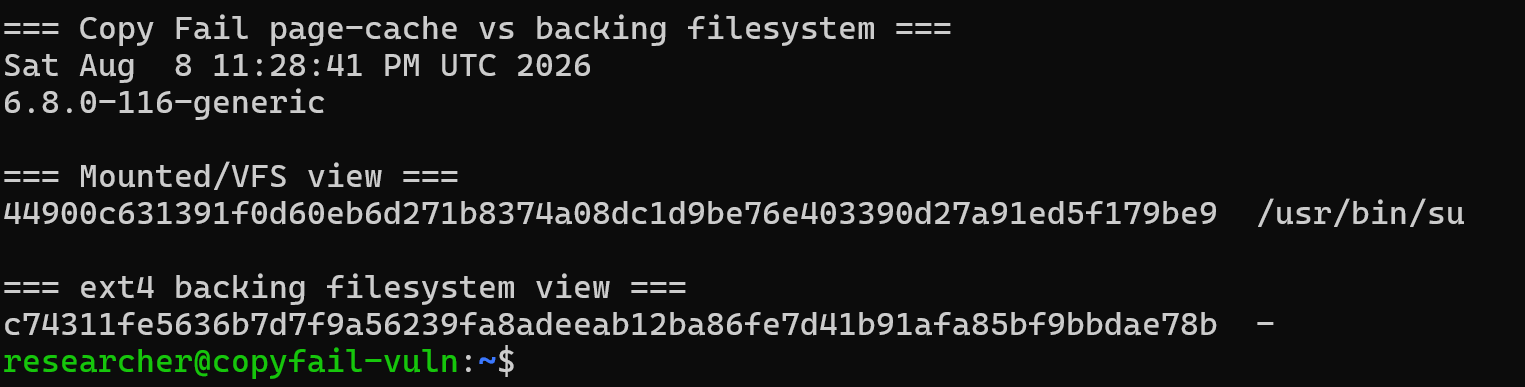
\includegraphics[
        width=\textwidth,
        height=0.31\textheight,
        keepaspectratio
    ]{02-reproduction/screenshots/06-page-cache-vs-backing-filesystem.png}
    \caption{Phase~02 comparison in which the mounted/VFS path returns the
    changed digest while the direct ext4 read returns the original digest.}
    \label{fig:phase02-view-divergence}
\end{figure}

The mounted/VFS read returned the changed digest recorded after exploitation,
while the ext4 read returned the original pre-exploitation digest. The two
access paths therefore produced different byte streams at the comparison point.
That observation is consistent with the published Copy Fail mechanism, where
file-backed cached data can be modified without the same change being written
back to the filesystem \cite{copyfail-research}.

The artifact proves the divergence, not the complete internal explanation. No
kernel instrumentation recorded page objects, dirty flags, scatterlists, or
writeback decisions during this step. The \code{debugfs} command was also a
live point-in-time read, not an offline forensic image. The strongest direct
conclusion is therefore that the mounted and backing-filesystem access paths
returned different content under the tested conditions.

\subsection{Recovery After Reboot}

The final phase recorded the target after rebooting into the same vulnerable
kernel. The screenshot captured at \code{2026-08-08 23:30:53 UTC} shows
\code{6.8.0-116-generic} still active and the mounted path once again returning
the original digest.

\begin{figure}[H]
    \centering
    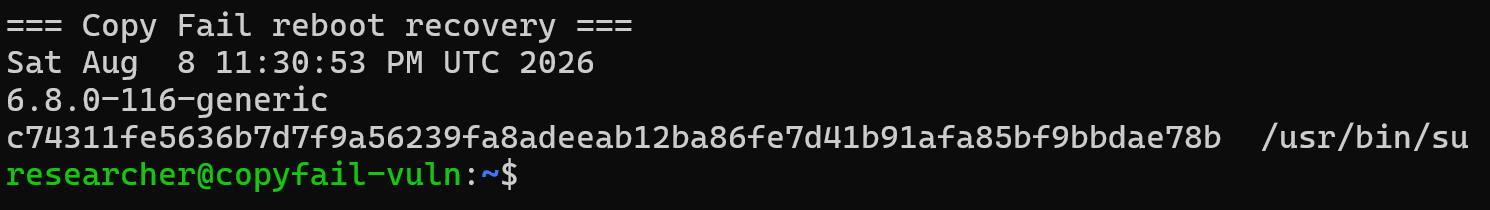
\includegraphics[
        width=\textwidth,
        height=0.22\textheight,
        keepaspectratio
    ]{02-reproduction/screenshots/07-reboot-restores-original-file.png}
    \caption{Post-reboot observation showing the original mounted-view digest
    on the same vulnerable kernel release.}
    \label{fig:phase02-reboot-recovery}
\end{figure}

A later text artifact, timestamped \code{2026-08-08 23:36:42 UTC}, records the
same release and digest and additionally confirms that the target had returned
to its original size, ownership, and SUID mode. These are two post-reboot
observations, not two representations of one simultaneous command.

Because the running release remained \code{6.8.0-116-generic}, the recovery did
not depend on installing a corrected kernel. Under the tested conditions, the
reboot cleared the previously visible mounted-view divergence while the
original backing content remained available.

Recovery is not remediation. The vulnerable kernel and normally loadable module
path were still present, so the prerequisites for another attempt could be
recreated. The recovery captures also do not include a boot identifier, uptime
comparison, or reboot-journal excerpt. They directly establish the recorded
post-reboot state; the reboot event itself is supplied by the documented
experimental sequence.

\subsection{Reproduction Result and Answer to RQ1}

The preserved sequence records a clear before, execution, and recovery path.
VM~271 began on the reconstructed \code{6.8.0-116-generic} runtime with
\code{labuser} at UID~1001 and the selected root-owned SUID target at its
original mounted-view digest. The separate laboratory operator loaded the
required modules. The proof of concept was then launched from the
\code{labuser} prompt, and the resulting shell returned UID~0 and
\code{root}.

\begin{table}[H]
    \centering
    \caption{Claim-to-evidence summary for the controlled reproduction.}
    \label{tab:phase02-findings}
    \small
    \begin{tabularx}{\textwidth}{@{}>{\bfseries\raggedright\arraybackslash}p{0.22\textwidth}>{\raggedright\arraybackslash}p{0.31\textwidth}Y@{}}
        \toprule
        Finding & Direct support & Boundary \\
        \midrule
        Vulnerable runtime active &
        Running release and matching \code{6.8.0-116.116} package records &
        The classification applies to the tested Ubuntu Noble configuration. \\

        Non-root starting identity &
        Item~01 records \code{labuser} at UID~1001 with the ordinary
        \code{users} group &
        The listing records the selected account state, not every possible
        privilege mechanism in the guest. \\

        UID~0 transition &
        Item~03 records \code{id} and \code{whoami} returning UID~0 and
        \code{root} &
        Screenshot-only evidence; the primary group remained GID~1001. \\

        Mounted view changed &
        Items~03 and~05 record the changed target digest &
        A changed digest does not identify the altered bytes or prove on-disk
        replacement. \\

        Read paths diverged &
        Item~06 records different mounted/VFS and ext4-read digests &
        Internal cache and writeback state were not instrumented directly. \\

        Original view recovered &
        Item~07 records the original digest on the same release after the
        declared reboot &
        Recovery does not correct the vulnerable kernel. \\
        \bottomrule
    \end{tabularx}
\end{table}

RQ1 asks whether Copy Fail can be reproduced in the isolated laboratory by an
ordinary, unprivileged local user. For the tested configuration, the answer is
yes. The preserved run starts from the dedicated UID~1001 account and records
the proof-of-concept command producing a UID~0 shell. That identity transition,
not the changed target digest, is the decisive result.

The scope remains deliberately narrow. The preliminary and preserved sequences
show operational repeatability on the same reconstructed VM, but the evidence
does not provide a multi-host trial matrix, a success-rate calculation, or a
statistical timing analysis. The result demonstrates the vulnerability under
the documented conditions; it does not quantify reliability across other
kernels, hardware, workloads, or timing states.

The digest sequence supplies the behavioural context needed for the next stage.
Chapter~6 examines which parts of this activity are observable, which signals
are specific enough to be useful, and how the experiment can move from a
successful reproduction to defensible detection logic.